\documentclass[12pt]{report}

\usepackage[left=1in, right=1in, top=1in, bottom=1in]{geometry}
\setlength\parindent{0pt}

\usepackage{graphicx, amsmath,anonchap,tabularx, multicol,verbatim}

\usepackage{enumitem,mdwlist}
\setlist{noitemsep}
\setlist{nolistsep}

\newenvironment{boxe}
    {\begin{center}
    \begin{tabular}{|p{0.9\textwidth}|}
    \hline\\
    }
    { 
    \\\\\hline
    \end{tabular} 
    \end{center}
    }

\begin{document}
\begin{tabular*}{\textwidth}{@{\extracolsep{\fill}}ll}
\textbf{Math 160} Continuity & \;\;Name: \hrulefill \\
 Hughes-Hallet Chapter 1.7& Continuity and the Intermediate Value Theorem\hspace{1in}  \\
\hline\hline
\end{tabular*} \\

\pagenumbering{gobble}





 \begin{boxe}
\textbf{Definition of Continuity}: A function $f$ is continuous at $x=c$ if and only if 
$$\lim_{x\rightarrow c}f(x)=f(c)$$
This implies that there are $3$ requirements for $f$ to be continuous at $x=c$
\begin{enumerate}
    \item The the function $f(x)$ evaluated at $c$ exists ($f(c)$ exists)
    \item The limit of $f(x)$ as $x$ approaches $c$ exists ($\lim_{x\rightarrow c}f(x)$ exists)
    \item The value of $f(c)$ and the value limit are the same ($\lim_{x\rightarrow c}f(x)=f(c)$)
\end{enumerate}
\end{boxe}
\begin{enumerate}
\item Consider the following graph for the function $f(x)$\\
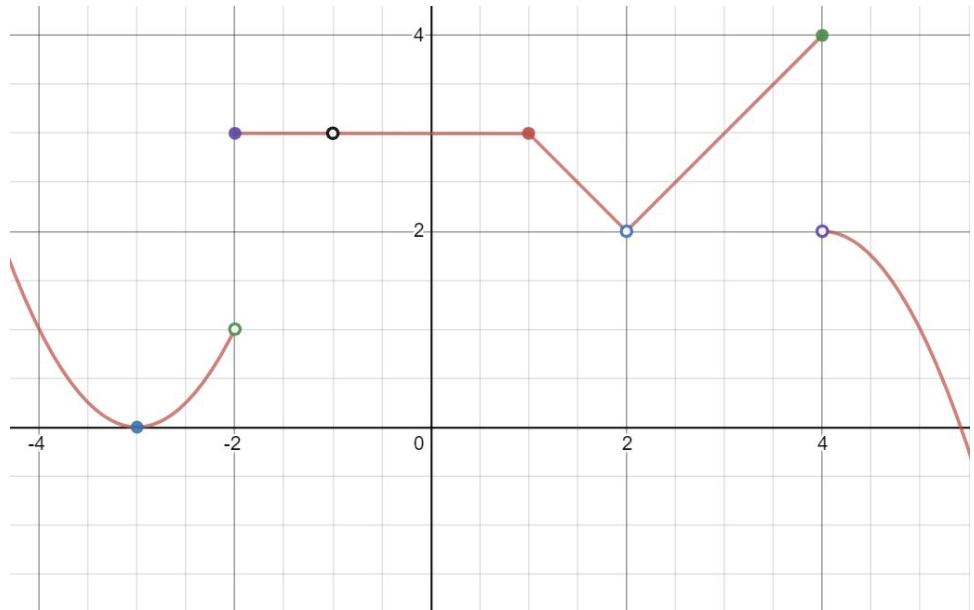
\includegraphics[scale=0.5]{ctsornot.png}\\
Explain why each of the following are true - support your answer. (You may approximate the values of limits graphically)\\
\begin{enumerate}[label=\alph*.]
    \item $\lim_{x\rightarrow 2}=2$\\\\\\\\\\
    \item The function $f(x)$ is continuous at $x=1$\\\\\\\\\\
    \item The function $f(x)$ is not continuous at $x=-2$
\end{enumerate}
\newpage

    \item Is $\displaystyle h(x) = \frac{3x^2+5x+2}{x+1}+\frac{e^x}{x}$ continuous at $x =-1?$ Use the definition of continuity to justify your answer. What $x$-values is $h(x)$ discontinuous at? Name the types of discontinuities.

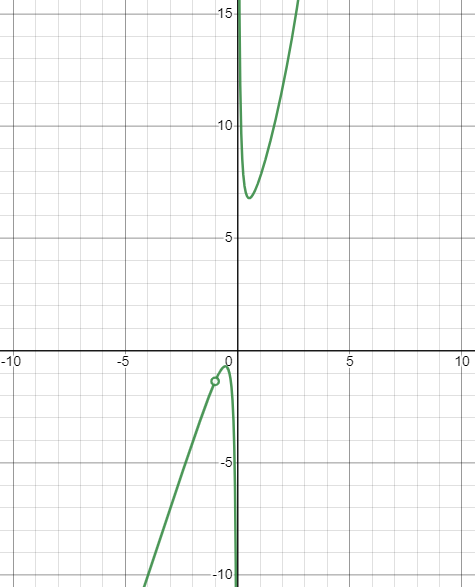
\includegraphics[scale=0.5]{contivtexplot.png} \\



\end{enumerate} 
 \begin{boxe}
\textbf{Intermediate Value Theorem}: Suppose $f$ is continuous on a closed interval $[a,b]$. If $u$ is any number between $f(a)$ and $f(b)$, then there is at least one number $c$ in $[a,b]$ such that $f(c)=u$.
\end{boxe}
\begin{enumerate}[resume*]
\item Consider the function $f(x)=x^{6}-2x^{5}+\frac{1}{2}x^{4}-2x^{2}-1$. Explain why each of the following are true - support your answers.\\
\begin{enumerate}[label=\alph*.]
    \item The function $f(x)$ has at least one root between $x=-2$ and $x=0$. (Recall that a root is an $x$-value $c$ where $f(c)=0$)\\\\\\\\\\
    \item The function $f(x)$ achieves the value $-2$ between $x=-1$ and $x=2$. (hint: you may need to use different values for $a$ in $b$)
\end{enumerate}









% commented out
\iffalse\subsubsection*{The 4 Types of Discontinuity}

\begin{itemize}
\item Removable (or hole) When x=-4, there is a hole. In theory, we could "remove" this discontinuity by filling in the hole. The limit exists but the function does not.
\item Jump- when x=2 there is a jump from one piece of the function to the next- the limit doesn't exist.
\item Infinite- when x=-1 there is a vertical asymptote with the function pieces tending toward positive or negative infinity. The limit doesn't exist.
\item Infinite Oscillation- the closer x gets to 5, the faster the function oscillates. It oscillates so quickly that there is no one value that we can approximate as accurately as desired by making x close to 5, so there is no limit.  For example, the function could be similar to $f\left(x\right)=\sin\left(\frac{1}{x}\right)$.
\end{itemize}

\includegraphics[scale=0.5]{ctytypes.png}

Continuity on an Interval

A function is continuous at a point x=c if the limit as x approaches c is equal to the value of the function when x=c.

We can extend this idea to discuss continuity of a function on an interval:

A function is continuous on an interval if it is continuous  at every point in the interval.

\vskip .1in

Side note about domains
When mathematicians talk about functions being continuous, they usually are only considering the domain of the function. Thus the following two statements are both true:

$\frac{1}{x}$ is continuous on its domain.

$\frac{1}{x}$ is discontinuous at x=0.

\newpage

Commonly used Continuous Functions
Here is a list of some common functions that are continuous (on their domains):

\begin{itemize}
\item linear functions ($y=mx+b$), parabolas ($y=ax2+bx+c$), and all polynomials
\item $\sin(x)$ and $\cos(x)$
\item $e^x$
\item $\sqrt{x}$ (for $x\geq0$) and $\ln(x)$ (for $x>0$)
\end{itemize}


Knowing these functions are continuous will be useful to us throughout the semester.

\vskip .5in

\item Construct examples of functions (a graph is fine, or a formula) that fit the following, or explain why such an example is not possible.

\begin{enumerate}
    \item A function that has a limit at $x = c$ but is NOT continuous at $x=c$.
    \vspace{1.5in}
    \item A function that is continuous at $x=c$ but does NOT have a limit at $x=c$.
    \vspace{1.5in}
    \item A function that has a limit at $x = c$ but is NOT defined at $x=c$.    \vspace{1.5in}
   \item A function that has a limit at $x = c$ and IS defined at $x=c$.    \vspace{1.5in}
\end{enumerate}



\fi
\end{enumerate}



\end{document}
